\documentclass[twoside]{article}
\usepackage{verbatim}
\usepackage{multirow} \usepackage{enumerate}
\usepackage{amsmath,enumerate} \usepackage{amsthm}
\usepackage{algcompatible}
\usepackage{algpseudocode}
\usepackage{algorithm}
%\usepackage{algorithmic}
%\usepackage{pstricks}
\usepackage{amssymb, latexsym}
\usepackage{xfrac}
\usepackage{mathtools}
\usepackage{graphicx}
\usepackage[captionskip=5pt, nearskip=5pt, font=small]{subfig}
\DeclareGraphicsRule{*}{mps}{*}{}
\usepackage{listings}

%specific to this document only
%\usepackage{pgfplots}
\usepackage{pgfplotstable}
\pgfplotstableread{plts/experiment_erdren_edgecolor.tab}\erdrenone
\pgfplotstableread{plts/experiment_erdren_edgecolor_400.tab}\erdrentwo
\pgfplotstableread{plts/experiment_erdren_directededgecolor.tab}\erddirone
\pgfplotstableread{plts/experiment_erdren_directededgecolor_400.tab}\erddirtwo
\pgfplotstableread{plts/experiment_sclfre_edgecolor.tab}\sclfreeone
\pgfplotstableread{plts/experiment_sclfre_edgecolor_400.tab}\sclfreetwo
\pgfplotstableread{plts/experiment_smlwld_edgecolor.tab}\smlwldone
\pgfplotstableread{plts/experiment_smlwld_edgecolor_64.tab}\smlwldtwo
\pgfplotstableread{plts/experiment_smlwld_edgecolor_256.tab}\smlwldthree
%\pgfplotstableread{plts/experiment8b2_av.tab}\averagetwo
%\pgfplotstableread{plts/experiment8b3_av.tab}\averagethree
%\pgfplotstableread{plts/experiment8b4_av.tab}\averagefour
%\pgfplotstableread{plts/experiment9a_av.tab}\stepping
%\pgfplotstableread{plts/experiment9a1_av.tab}\steppingone
%\pgfplotstableread{plts/experiment9a2_av.tab}\steppingtwo
%\pgfplotstableread{plts/experiment9a3_av.tab}\steppingthree
%\pgfplotstableread{plts/experiment9a4_av.tab}\steppingfour
%\pgfplotstableread{plts/experiment9b1_av.tab}\runningone
%\pgfplotstableread{plts/experiment9b2_av.tab}\runningtwo
%\pgfplotstableread{plts/experiment9b3_av.tab}\runningthree
%\pgfplotstableread{plts/experiment9b4_av.tab}\runningfour
%\pgfplotstableread{plts/experiment9b_av.tab}\running
%\pgfplotstableread{plts/experiment9c_av.tab}\costcomp
%\pgfplotstableread{plts/experiment9c1_av.tab}\costcompone
%\pgfplotstableread{plts/experiment9c2_av.tab}\costcomptwo
%\pgfplotstableread{plts/experiment9c3_av.tab}\costcompthree
%\pgfplotstableread{plts/experiment8b1_rn.tab}\runsone
%\pgfplotstableread{plts/experiment8b2_rn.tab}\runstwo
%\pgfplotstableread{plts/experiment8b3_rn.tab}\runsthree
%\pgfplotstableread{plts/experiment8b4_rn.tab}\runsfour
%\pgfplotstableset{
%  create on use/density/.style={
%    create col/expr={\thisrow{nodes}+\thisrow{links}}}
%    }
\pgfplotstableset{
  create on use/delta/.style={
    create col/expr={\thisrow{links}/\thisrow{nodes}}
    }}
%\pgfplotstableset{
%  create on use/nodebylinks/.style={
%    create col/expr={(\thisrow{nodes}*\thisrow{links})}}
%    }
%\pgfplotscreateplotcyclelist{three}{% 
%  every mark/.append style={fill=teal}\\% 
%  every mark/.append style={fill=green}\\% 
%  every mark/.append style={fill=orange}\\% 
%}
%\pgfplotscreateplotcyclelist{four}{%
%  every mark/.append style={fill=teal}\\%
%  every mark/.append style={fill=green}\\%
%  every mark/.append style={fill=orange}\\%
%  every mark/.append style={fill=pink}\\%
%}
%\pgfplotscreateplotcyclelist{three-1-0}{%
%  every mark/.append style={fill=teal}\\% 
%  every mark/.append style={fill=green}\\% 
%  every mark/.append style={fill=orange}\\%
%	every mark/.append style={fill=none}\\% 
%	every mark/.append style={fill=none}\\% 
%	every mark/.append style={fill=none}\\% 
%}
%\pgfplotscreateplotcyclelist{three-0-1}{%
%	every mark/.append style={fill=none}\\% 
%	every mark/.append style={fill=none}\\% 
%	every mark/.append style={fill=none}\\% 
%  every mark/.append style={fill=teal}\\% 
%  every mark/.append style={fill=green}\\% 
%  every mark/.append style={fill=orange}\\%
%}
%\pgfplotscreateplotcyclelist{four-1-0}{%
%  every mark/.append style={fill=teal}\\%
%  every mark/.append style={fill=green}\\%
%  every mark/.append style={fill=orange}\\%
%  every mark/.append style={fill=pink}\\%
%	every mark/.append style={fill=none}\\%
%	every mark/.append style={fill=none}\\%
%	every mark/.append style={fill=none}\\%
%	every mark/.append style={fill=none}\\%
%}
%\pgfplotscreateplotcyclelist{four-0-1}{%
%	every mark/.append style={fill=none}\\%
%	every mark/.append style={fill=none}\\%
%	every mark/.append style={fill=none}\\%
%	every mark/.append style={fill=none}\\%
%  every mark/.append style={fill=teal}\\%
%  every mark/.append style={fill=green}\\%
%  every mark/.append style={fill=orange}\\%
%  every mark/.append style={fill=pink}\\%
%}

%%%%%%%%%%%%%

\usepackage{pgf}
\usepackage{tikz}
\usetikzlibrary{decorations.pathmorphing} % LATEX and plain TEX when using Tik Z
\usetikzlibrary{positioning}
\usetikzlibrary{er}
\usetikzlibrary{automata}
\usetikzlibrary{shapes.geometric}
\usetikzlibrary{shapes.misc}
\tikzstyle{vx}=[draw,circle,fill=white,minimum size=2pt, inner sep=1pt, node distance=15mm]
\tikzstyle{ex}=[draw,rectangle,fill=white,minimum size=2pt, inner sep=3pt, node distance=15mm]
\tikzstyle{nfo}=[anchor=north west, rectangle, fill=white,text width=4cm, inner sep=3pt, node distance=15mm]
\tikzstyle{bup}=[semithick, decoration={bent, aspect=.3, amplitude=4}, decorate, ->, >=stealth]
\tikzstyle{bdn}=[semithick, decoration={bent, aspect=.3, amplitude=-4}, decorate, ->, >=stealth]
\tikzstyle{BUP}=[thick, decoration={bent, aspect=.3, amplitude=8}, decorate, ->, >=stealth]
\tikzstyle{BDN}=[thick, decoration={bent, aspect=.3, amplitude=-8}, decorate, ->, >=stealth]
\tikzstyle{MUP}=[thick, decoration={bent, aspect=.3, amplitude=16}, decorate, ->, >=stealth]
\tikzstyle{MDN}=[thick, decoration={bent, aspect=.3, amplitude=-16}, decorate, ->, >=stealth]
\tikzstyle{pln}=[draw, dotted]
\tikzstyle{dir}=[draw, dotted, decorate, ->, >=stealth, bend left=10]
\tikzstyle{str}=[semithick, decorate, ->, >=stealth]
\tikzstyle{cr}=[draw, circle, fill=black!25,minimum size=150pt]
\tikzstyle{rst}=[state, shape=rounded rectangle, rounded rectangle arc length=90, text width=2cm, inner sep=4pt]
\tikzstyle{rsf}=[state, fill=green!35, shape=rounded rectangle, rounded rectangle arc length=90, text width=1.75cm, inner sep=4pt]
%styles for plots?
\tikzstyle{bls}=[blue, solid, mark=square*]
\tikzstyle{grt}=[red, solid, mark=*]
\tikzstyle{inv}=[draw=none]

% \paperheight=11in \paperwidth=8.5in \textheight=9.0in
% \textwidth=6.5in \voffset=-.875in \hoffset=-.875in
\newenvironment{code} {\begin {quote}\begin{footnotesize}}
    {\end{footnotesize}\end{quote}}

% \oddsidemargin 0.0 in \evensidemargin 0.0 in
\newenvironment{enumeratealpha}
{\begin{enumerate}[(a{\textup{)}}]}{\end{enumerate}}

\theoremstyle{plain}
\newtheorem{lem-rule}{Rule}
\newtheorem{thm}{Theorem}
\newtheorem{con}{Conjecture}
\newtheorem{lem}{Lemma}[thm]
\newtheorem{prp}{Proposition}
\newtheorem{prop}{Proposition}[con]
\newtheorem{lprp}{Proposition}[lem]
\newtheorem{cor}{Corollary}[lem]
\theoremstyle{definition}
\newtheorem{defn}{Definition}[thm]
\newtheorem{defi}{Definition}
\newtheorem{dfn}{Definitions}[thm]
\newtheorem{ldef}{Definition}[lem]
\newtheorem{assm}{Assumption}
\theoremstyle{remark}
\newtheorem*{smy}{Summary}
\newtheorem{note}{Note}[thm]
\newtheorem{case}{Case}
%algorithms commands
\algblockdefx[Case]{Case}{EndCase} %
[1] [{\em var}] {{\bfseries case} {\em #1\ } } %
{{\bfseries end case}}%
\algcblockdefx[Case]{Case}{When}{EndCase}
[1] [{\em true}] {{\bfseries when} {\em #1\ }}
{{\bfseries end case}} %

\algblockdefx[TimesDo] {DoTimes}{EndTimes}
[1] [0] {#1 times {\bfseries do}}
{{\bfseries end do}}

%subalgorithms environment
\makeatletter
\newcounter{parentalgorithm}
\newenvironment{subalgorithms}{%
%  \refstepcounter{algorithm}%
  \floatname{algorithm}{Procedure}
  \protected@edef\theparentalgorithm{\thealgorithm}%
  \setcounter{parentalgorithm}{\value{algorithm}}%
  \setcounter{algorithm}{0}%
  \def\thealgorithm{\theparentalgorithm-\alph{algorithm}}%
  \ignorespaces
}{%
  \setcounter{algorithm}{\value{parentalgorithm}}%
  \ignorespacesafterend
}
\makeatother

%code environments
\usepackage{float}
 
\floatstyle{ruled}
\newfloat{codeblock}{thp}{lop}
\floatname{codeblock}{Example}

\lstnewenvironment{rubyblock} 
{\lstset{language=Ruby, breaklines=true, basicstyle=\small, xleftmargin=10pt, numbers=left, numberstyle=\tiny, stepnumber=1, numbersep=5pt, escapeinside={|;}{;|}}}
{}
% text macros
\def\cI{{\mathcal I}} \def\cR{{\mathcal R}} \def\cE{{\mathcal E}}
\def\cC{{\mathcal C}} \def\cF{{\mathcal F}} \def\cU{{\mathcal U}}
\def\cH{{\mathcal H}} \def\cD{{\mathcal D}} \def\cB{{\mathcal B}}
\def\cQ{{\mathcal Q}} \def\cV{{\mathcal V}} \def\cS{{\mathcal S}}
\def\cG{{\mathcal G}} \def\cA{{\mathcal A}} \def\cO{{\mathcal O}}
\def\cW{{\mathcal W}} \def\cL{{\mathcal L}} 

\def\bI{{\mathbb I}} \def\bO{{\mathbb O}}
\def\bC{{\mathbb C}} \def\bM{{\mathbb M}}
\def\bId{{$\mathbb I$}} \def\bOd{{$\mathbb O$}}
\def\bCd{{$\mathbb C$}} \def\bMd{{$\mathbb M$}}

\def\cId{{$\mathcal I$}} \def\cRd{{$\mathcal R$}} \def\cEd{{$\mathcal E$}} 
\def\cCd{{$\mathcal C$}} \def\cFd{{$\mathcal F$}} \def\cUd{{$\mathcal U$}} 
\def\cHd{{$\mathcal H$}} \def\cDd{{$\mathcal D$}} \def\cBd{{$\mathcal B$}} 
\def\cQd{{$\mathcal Q$}} \def\cVd{{$\mathcal V$}} \def\cSd{{$\mathcal S$}} 
\def\cGd{{$\mathcal G$}} \def\cAd{{$\mathcal A$}} \def\cOd{{$\mathcal O$}}
\def\cWd{{$\mathcal W$}} \def\cLd{{$\mathcal L$}}

\def\suchthat{{\: |\:}}




\usepackage{IJNC}


\setcounter{page}{501}
\newcommand{\jvolume}{X}
\newcommand{\jnumber}{Y}
\newcommand{\jmonth}{January}
\newcommand{\jyear}{20XX}

% title
\newcommand{\jtitle}{A General Purpose Automata for Distributed Graph Algorithms}
% running title for header
\newcommand{\jrunningtitle}{A General Purpose Automata}



\pagestyle{plain}


\begin{document}
\thispagestyle{empty}
\copyrightheader

\begin{center}
% print title
\jtitle

\vspace{20pt}

J. Paul Daigle 

\vspace{2pt}

Department of Computer Science, Georgia State University\\
Atlanta, GA, 30303, USA

\vspace{10pt}
%and
%
\vspace{10pt}
Sushil K. Prasad

\vspace{2pt}
Department of Computer Science, Georgia State University\\
Atlanta, GA, 30303, USA

\vspace{10pt}
%and
%
%\vspace{10pt}
%THIRD AUTHOR
%
%\vspace{2pt}
%Group, Laboratory, Address\\
%City, State ZIP, Country

\vspace{20pt}
\publisher{(received date)}{(revised date)}{(accepted date)}{Editor's name}
%\publisherA{(received date)}{(revised date)}{(revised date)}{(accepted date)}{Editor's name}

\end{center}


\begin{abstract}
We present an automata for a compute node in a message passing model which allows a distributed computer to approximate solutions for three NP-Complete graph problems. Our algorithm for the Vertex Cover Problem uses $O(\log{\Delta)}$ communication rounds to find a 2-approximate solution. Our edge coloring algorithm is also 2-approximate and resolves in $O(\Delta)$ rounds, and we find a correct strong edge coloring of a symmetric digraph in $O(\Delta)$ rounds. All three algorithms require only one hop information to find correct solutions. 
\keywords{Distributed Algorithms, Vertex Cover, Edge Coloring, Strong Edge Coloring}
\end{abstract}


\section{Introduction}

In this paper we expand on our prior work in \cite{Daigle:2011uq, Daigle:2012uq} using a simple Matching Automata to find constant approximations for NP-complete problems on a message passing computer. We present both theoretical and experimental results. We improve on our prior work in two ways, first, we improve our proof for correctness and performance, second, we present expanded experimental results, and third, we present an improved algorithm for edge color.


\subsection{Definitions}

\begin{defi}[Minimum Vertex Cover]
\label{sub:mvc}

Given an undirected Graph $G(V,E)$, a {\em Vertex Cover} of $G$ is a set of vertices $V'$ such that for each edge $e_{u,v} \in E$, $u \in V'$ or $v \in V'$. The Minimum Vertex Cover Problem is to find the smallest possible vertex cover of $G$.

\end{defi}

\begin{defi}[Minimum Weighted Vertex Cover]
\label{sub:mwvc}
Given an undirected Graph $G(V,E)$, where each $v \in V$ has a positive weight $w(v)$, minimize $\sum_{v \in V'} w(v)$.
\end{defi}

\begin{defi}[Edge Coloring]
\label{def:ec}
An edge coloring of a graph is an assignment of colors to the edges of a graph in such a way that no two adjacent edges are assigned the same color. 

Formally, given a graph, $G(V,E)$, and set of colors $C$, an edge coloring of $G$ is a mapping $f(e) = E \mapsto C \suchthat \forall\, e(u,v), e'(v,w) \in E, c \in C, f(e) = c \implies f(e') \ne c$.

\end{defi}


\begin{defi}[Strong Directed Edge Coloring]

A strong edge coloring is an assignment of colors to the edges of the graph such that no two edges that can be connected by a common edge are assigned the same color. 

In the directed case, a strong edge coloring is a mapping:
  \begin{align*} 
    f(e) = C \mapsto E \suchthat \forall\, e(u,v), e'(v,u), e''(w,v), e'''(w,x) \in E, c \in C,\\ 
    f(e) = c \implies f(e') \ne c, f(e'') \ne c, f(e''') \ne c 
  \end{align*} 
\end{defi}


\subsection{The Model and Automata}

\subsubsection{The Message Passing Model}
Our algorithms assume a message passing model of distributed computing. Therefore, we make the following two assumptions. First, communication rounds proceed synchronously. Second, each node can communicate with each of its neighbors once during any communication round. Structurally, our algorithms map each vertex of the graph to a compute node of the distributed computer. 

We also use the term `round' in two different senses. A computation round in our algorithm is composed of several communication rounds. Referring to the automata in Figure~\ref{fig:automata}, the automata defines the possible states of a node during a single computation round. We describe these steps in more detail in Section~\ref{sec:framework}.

A key point is that nodes are assumed to move synchronously through the stages of the automata regardless of whether they send or recieve messages in any given phase. We place certain restrictions on what computations a node will make and on what messages a node will consider addressed to itself in any given round, but our model does not rely on such messages to keep the nodes moving forward.

The purpose of the our framework is to generate a matching\footnote{A matching for a graph $G(V,E)$ is a subset $E' \subset E \suchthat \forall\, e(u,v), e'(u,w), e''(v,x) \in E, e \in E' \implies e' \notin E', e'' \notin E'$. Less formally, no two contiguous edges are in the matching.} on the graph in each computation round. For a number of graph problems, including edge coloring and vertex cover, finding such a matching allows for local computations to be made simultaneously by the nodes in the matching without the possibility of conflict.  

\subsubsection{The Matching Automata}
\label{sec:automata}
Our framework relies on a simple handshake protocol, represented by the state machine in Figure~\ref{fig:automata}.

Our approach is to have all of the compute nodes participate in forming a matching $V' \subset V$. The first three steps of the automata show our method for forming this matching. Having formed the matching, the nodes that are in $V'$ compute local solutions and broadcast them to all of their neighbors. This continues until every necessary local solution has been found. 
\begin{figure}[htp]
  \begin{center}
  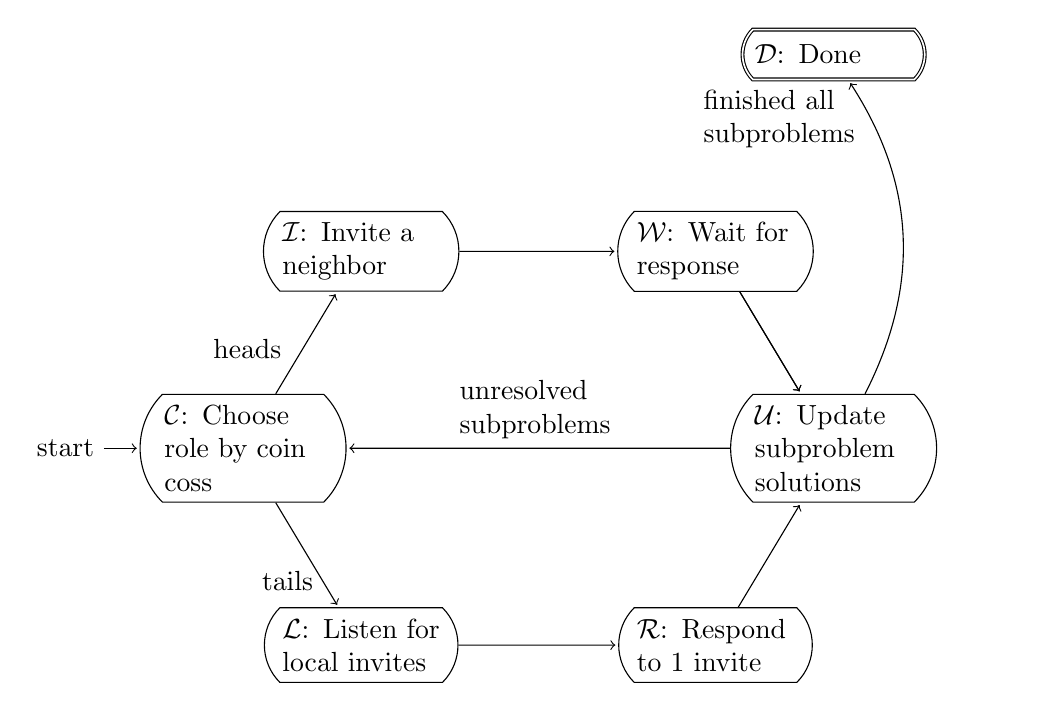
\begin{tikzpicture}[shorten >=1pt,node distance=1cm,on grid,auto, bend angle=75, every state/.style={scale=1, minimum size=18pt, inner sep=2pt}]
    %\draw [help lines] (-5,-4) grid (7,4);
    \path [help lines] (-4,-4) grid (7,4);
		
    \node [rst, initial]   (C) at (-3,-1) {\cCd: Choose role by coin coss};
    \node [rst] (I)            at (-1.5,1.5) {\cId: Invite a neighbor};
    \node [rst] (L)            at (-1.5,-3.5) {\cLd: Listen for local invites};
    \node [rst] (W)            at (3,1.5)  {\cWd: Wait for response};
    \node [rst] (R)            at (3,-3.5) {\cRd: Respond to 1 invite};
    \node [rst] (U)            at (4.5,-1) {\cUd: Update subproblem solutions};
    \node [rst, accepting] (D) at (4.5,4)  {\cDd: Done};

    \path [->] (C) edge              node [near start] {heads} (I)
               (C) edge              node [near end, left] {tails} (L)
               (L) edge              node {} (R)
               (I) edge              node {} (W)
               (W) edge              node {} (U)
               (R) edge              node {} (U);
    \path [->] (U) edge [bend right=30]             node [very near end, left, text width=2cm] {finished all subproblems} (D);
    \path [->] (W) edge  node {} (U);
    \path [->] (U) edge  node [above, text width=2cm] {unresolved subproblems} (C);

  \end{tikzpicture}
  \caption{Distributed Matching and Computation Automata}
  \label{fig:automata}
  \end{center}
\end{figure}


Each node begins a decision round in the \cCd, or {\em choose} state, and chooses randomly whether to transition to the \cId\ or \cLd\ state. Nodes in the \cId\ state choose a single neighbor with a shared subproblem (such as covering or coloring a shared edge) and issue an {\em invitation} to solve that subproblem in this round. 

An invitation should contain all of the information that the invitee needs to compute the solution to the subproblem for this round. For example, if the problem being solved is edge coloring, a node would send it's own id, the id of the intended receiver, and a set of potential colors. Nodes in the \cLd\ state collect any invitations addressed to them. 

In the next step, each node that was in the \cLd\ state transitions to the \cRd\ state, chooses a single invitation from their collection and responds to that invitation. An invitation response is essentially a mirror of the original invitation, containing the id of the responding node, the id of the original sender, and an acceptable solution to the subproblem. 

Nodes in the \cId\ state transition to \cWd\ state and filter incoming messages for the response to the invitation that they sent in the previous step. 

Finally, all nodes transition to the \cUd\ state, solve their local subproblem, and broadcast their solutions. Nodes with no outstanding problems to be solved transition to \cDd\ and terminate, nodes with outstanding sub-problems go back to \cCd.


\subsection{Prior Work}

\subsubsection{Vertex Cover}

Sequential Linear time algorithms for covering problems are surveyed in detail in \cite{254190}. The seminal paper on Linear Programming techniques for constant ratio approximation of MWVC was published by Bar-Yehuda and Even in 1981 \cite{Bar-Yehuda:1981lr}. Gonzalez created a 2-approximate LP-Free linear time algorithm based on Maximal Matching in 1995 which is the basis of our distributed algorithm \cite{Gonzalez1995129}. 

We are aware of three prior distributed algorithms for minimum weighted vertex cover. Grandoni et. al present a 2-approximate algorithm based on maximal matching in 2008\cite{1435381}. This algorithm uses $O(\log n + \hat{W})$ communication rounds, where $\hat{W}$ is the average vertex weight, and $n$ is the number of vertexes. {\AA}strand and Suomela presented a $O(\Delta + \hat{W})$ deterministic algorithm in 2010 which is also 2-approximate. Koufogiannakis and Young present a simpler $O(\log n)$ algorithm in 2009 \cite{1582746}. 

Parnas and Ron proved in 2007 that the query complexity of a randomized algorithm for solving MWVC in a message passing model grows linearly with the average degree of the graph\cite{Parnas:2007:AMV:1280283.1280327}. Following that work, Onak, Ron, Rosen and Rubinfeld present a deterministic algorithm that is 2-approximate in $O(\delta)$ time, where $\delta$ is the average degree of the graph\cite{Onak:2012:NSA:2095116.2095204}. 


\subsubsection{Edge Coloring}

Distributed edge coloring is a well studied problem. Panconesi and collaborators have produced a number of papers tying edge coloring to channel assignment and presenting novel edge coloring algorithms with communication complexity of as low as $O(log{log{n}})$ \cite{Grable:1997:NOD:314161.314266},\cite{Panconesi:1997:RDE:249364.249368},\cite{1041515},\cite{982945}.

Gandham et al. present an deterministic algorithm which colors a graph using $\Delta + 1$ colors with a time complexity of $2\Delta + 1$ for acyclic graphs \cite{1498534}. Barenboim et al. present a deterministic algorithm which extends beyond trees and provides an $O(\Delta)$ coloring in $O(\Delta^{1 + \epsilon})$ time for an arbitrarily small constant $\epsilon \le 1$ \cite{Barenboim:2011:DDE:1993806.1993825}. A limitation of this algorithm is that the constant factor for quality increases as $\epsilon$ decreases.

In strong edge coloring, Barret et al. present algorithms with running times dependent on the size of the graph $n$ \cite{1598948}. Kanj et al. show tight bounds for the quality and locality, but not the time bounds, of their algorithms \cite{Kanj:2009:LAE:1696884.1696902}.


\section{The Vertex Cover Problem}

In this section we'll present the findings for Vertex Cover.

\subsection{Algorithm}
\label{sec:dgmm-description}

Algorithm~\ref{alg:dgmm} is our distributed implementation of the 2-optimal minimum weighted vertex cover algorithm presented by Gonzalez \cite{Gonzalez1995129}. The Gonzalez algorithm, Generalized Maximal Matching for MWVC (or GMM), proceeds by selecting each edge in turn and choosing one of the endpoints of that edge to add to the cover. The sequential algorithm goes through each edge in turn and assigns the edge a weight according to~\eqref{eqn:gmm}.

\begin{align}
  \label{eqn:gmm}
  w(e(u,v)) = min 
  \begin{dcases} 
    w(u) - \sum_{i \ne v} w(e(u,i)) \\
    w(v) - \sum_{i \ne u} w(e(i,v)) 
  \end{dcases} \nonumber \\ 
\intertext{where } 
   w(e(u,i))\text{ or } w(e(i,v)) = 0 \nonumber
\intertext{for unweighted edges}
\end{align}


So if there are no previously weighted edges incident to either endpoint, the weight of the edge is $min(w(u),w(v))$. A vertex $u$ joins the cover when, for all it's weighted edges: \begin{equation}\sum_i w(e(u,i)) = w(u) \label{eqn:sat} \end{equation} When~\eqref{eqn:gmm} is applied to subsequent unweighted incident edges of $u$, the result will be 0. The algorithm terminates when each edge has been weighted. 

In GMM, every edge is examined exactly once. If no endpoints of the edge are in the cover, one endpoint will join the cover. Finally, all the edges are evaluated in arbitrary order. We explore this third point further in Section~\ref{ssb:algorithms-dgmm-performance}. 

Our distributed version of the algorithm chooses some disjoint set of edges (a matching) and assigns weights to those edges according to~\eqref{eqn:gmm}. The framework automata is used to construct the set of disjoint edges in the following manner.\footnote{For the following description, we will substitute the symbol $\varpi(u)$ for the term $\sum_i w(e(u,i))$ in~\eqref{eqn:gmm}.\label{fn:varpi}}

Each node begins in the \cCd\ state. In the first step, each node chooses to transition to state \cId\ or \cLd\ with equal probability. Each node $u$ in the \cId\ state chooses an unweighted edge $e(u,v)$ at random, and broadcasts an invitation containing its incident edge weight ($\varpi(u)$)\footnotemark[\value{footnote}] and the edge it wants to weight. Each node $v$ in the \cLd\ state collects the invitations that contain an edge $e(i,v)$.

For the next step, nodes in the \cLd\ state transition to the \cRd\ state, and nodes in the \cId\ state transition to the \cWd\ state. Each node $v$ in the \cLd\ state chooses an invitation it collected in the prior step and issues a response containing $\varpi(v)$ and the edge $e(u,v)$ that it agrees to weight. Each node in the \cWd\ state filters these responses for the one containing an edge $e(u,i)$ (that is, a response to the invitation it sent in the prior round). 

At this point, there are a number of node pairs in the graph, every node $u$ that sent an invitation to weight an edge $e(u,v)$ forms a pair with $v$ if $v$ responds with an agreement to weight $e(u,v)$. The edges that will be weighted in this round are a matching.

Every node now transitions to the \cUd\ state. Those that have formed node pairs weight the edge $e(u,v)$ according to~\eqref{eqn:gmm}. One of $u,v$ will join the cover at this point. For brevity, in Algorithm~\ref{alg:dgmm}, the \cUd\ state is implied in lines~\algref{alg:dgmm}{alglin:dgmm-update-weight-R} and \algref{alg:dgmm}{alglin:dgmm-update-weight-W}.

Every node now transitions to the \cEd\ state, and broadcasts its current status to its neighbors. If a node $v$ receives a message that a neighbor $u$ has joined the cover $v$ will assign a weight of 0 to $e(u,v)$ and remove $e(u,v)$ from its list of unweighted edges. Again for brevity, the \cEd\ state is executed by implication in lines~\algref{alg:dgmm}{alglin:dgmm-state-E-W} and \algref{alg:dgmm}{alglin:dgmm-state-E}.

Every node that is in the cover now transitions to the \cDd\ state, as does any node that has no unweighted edges remaining. Nodes that still have unweighted edges go back to the \cCd\ state and repeat the process. 


\begin{algorithm}
\caption{Distributed Maximal-Matching-based Minimum-Weighted Vertex Cover  Algorithm (DGMM)}
\begin{algorithmic}[1]
%\Require {$G(V,E)$: a Communication Network}
\ForAll {$v_u \in V$ in parrallel}
\State $S_u \leftarrow False$ \Comment $u$ is not in the cover
\State state $\leftarrow$ \cCd
\Repeat
\State Broadcast $S_u$
\If {$S_v = True$ for $v_v$ incident to self}
\State Set Weight $e_{u,v} \leftarrow 0$ \label{alglin:dgmm-state-E}
\EndIf
\If {state = \cCd}
\State {State $\gets (\cI \lor \cL)$} \Comment Coin toss selects state
\ElsIf {state = \cId}
\State {Randomly select an unweighted edge, $e_{u,v}$}\label{alglin:dgmm-issue-invite}
\State {Broadcast $I_u^v\varpi(u)$} \Comment $u$ Invites $v$ to weight $e_{u,v}$ \label{alglin:dgmm-invite}
\State {state $\leftarrow$ \cWd}
\ElsIf {state = \cLd}
\State {Recieve $I_x^y$} \Comment all local invites
\If {$y = u$} \Comment invite is targeted to $v_u$
\State {store $I_x^y$}
\EndIf
\State {State $\gets \cR$}

\ElsIf {state = \cRd}
\State {Randomly Select $I_v^u$} \Comment from stored invites \label{alglin:dgmm-choose-invite}
\State {Broadcast $R_u^v$} \Comment $u$ accepts $v's$ invitation
\State {Update Weight $e_{u,v}$} \Comment by Equation~\ref{eqn:gmm} \label{alglin:dgmm-update-weight-R}

\If {$\sum w(e(i,u)) = w(u)$}\label{alglin:dgmm-join-cover-R}
\State {$S_u \gets true$} \Comment $u$ joins the cover
\State {Set all unweighted edges to 0} 
\State {state $\gets \cD$}
\Else 
\State {state $\gets \cC$}
\EndIf

\ElsIf {state = \cWd}
\State {Recieve $R_x^y$} \Comment all local responses

\If {$y = u$} \Comment response is to $v_u$
\State {Update Weight $e_{u,v}$}\label{alglin:dgmm-update-weight-W}

\If {$\sum w(e(i,u)) = w(u)$}\label{alglin:dgmm-join-cover-W}
\State $S_u \leftarrow true$ \Comment $u$ joins the cover
\State {Set all unweighted edges to 0}\label{alglin:dgmm-state-E-W}
\State {state $\leftarrow$ \cDd}
\Else 
\State {state $\leftarrow$ \cCd}
\EndIf

\EndIf

\EndIf

\Until {$S_u = true$ OR $S_v = true$  $\forall v_v$ incident $v_u$}\label{alglin:dgmm-end-while}
\EndFor
\end{algorithmic}
\label{alg:dgmm}
\end{algorithm}

\subsection{Analysis}

\label{ssb:algorithms-dgmm-performance}

Despite its overall simplicity, Algorithm~\ref{alg:dgmm} has a running time of $O(\log \Delta)$, which improves on the previous best result of $O(\log n)$ in \cite{1582746} without sacrificing the performance bound of two-optimality. A formal proof of our performance claims follows.

\begin{thm}
  Algorithm~\ref{alg:dgmm} (DGMM) will generate a 2-optimal cover in $O(log \Delta)$ communication rounds with high probability on random input.
\label{thm:dgmm-term}
\end{thm}

\begin{proof}[Proof of Theorem~\ref{thm:dgmm-term}]
\label{prf:correct}

\begin{lem}
\label{lem:dgmm-edge}
  DGMM weights each edge once in a manner equivalent to GMM.
\end{lem}


\begin{lem}
\label{lem:dgmm-log}
Algorithm~\ref{alg:dgmm} (DMMW) terminates in $O(log \Delta)$ rounds with high probability for random connected graphs.
\end{lem}


\begin{proof}[Proof of Lemma~\ref{lem:dgmm-log}]
\begin{ldef}
A node is {\em committed} if it has joined the cover or if all of its neighbors have joined the cover.
\end{ldef}
\begin{ldef}
A node is {\em active} if it is not committed.
\end{ldef}
\begin{ldef}
$\Delta$ is the maximum degree of the Graph.
\end{ldef}

\begin{ldef}
The active degree of a node $u$ is the number of unweighted edges of $u$ indicated by $\alpha(u)$. $\alpha(u)$ is either 0 for committed nodes or equal to the number of active neighbors of $u$ for active nodes.
\end{ldef}
\begin{ldef}
$\delta$ is the largest active degree in the graph.
\end{ldef}

Lemma~\ref{lem:dgmm-log} can be restated in terms of the following propositions:
\begin{lprp}
\label{prop:dgmm-log-each}
Each active node in the graph joins the cover with a constant probability in each round.
\end{lprp}
\begin{lprp}
\label{prop:dgmm-log-alpha}
With high probability, $\delta$ decreases by a constant fraction in each round.
\end{lprp}
\begin{proof}[Proof of Proposition~\ref{prop:dgmm-log-each}]

We begin with a node, $w$, which is an active node in the graph. We want to show that the probability that $w$ will join the cover is constant. Let us assume that $w$ chooses to be a receiver, an event which happens with $P(0.5)$

We know that $w$ has some number of active neighbors, indicated by $\alpha(w)$. Each neighbor of $w$ also has some number of active neighbors. Each active degree is an integer between 1 and $\delta$. We can consider each node to have approximately the same active degree, which we indicate by $\alpha$. 

Each active neighbor of $w$ also chooses to be a sender or a receiver with equal probability. Following the assumption of equal distribution, there are $\sfrac{\alpha}{2}$ senders in the neighborhood of $w$, and each sender has $\alpha$ neighbors.

Each neighbor of $w$ that chooses to be a sender will, according to Line~\ref{alglin:dgmm-issue-invite} of Algorithm~\ref{alg:dgmm}, choose one neighbor which is active and send an invitation to that node. Because there are approximately $\sfrac{\alpha}{2}$ inviting neighbors of $w$, we can consider the probability that $w$ will recieve an invitation to be approximately equivalent to the probability that any event with a probability of $\sfrac{1}{n}$ will occur in $\sfrac{n}{2}$ independent trials for $n > 0$. 

Therefore, the probability that $w$ will recieve an invitation from an active neighbor is: \begin{equation}
1 - \left(\frac{n-1}{n}\right)^{\frac{n}{2}} > \lim_{0 \to \infty} 1 - \left(\frac{k-1}{k}\right)^{\frac{k}{2}} = 1 - \frac{1}{\sqrt{{\mathrm{e}}}} \approx 0.393
\end{equation}


If $w$ recieves at least one invitation, it will respond to exactly one invitation (\algref{alg:dgmm}{alglin:dgmm-choose-invite}), so the probability that $w$ will respond to an invitation from some active neighbor $v$ is exactly the same as the probability that $w$ will recieve an invitation from some active neighbor $v$. Therefore, if $w$ is a receiver, $w$ joins the cover with a probability of $1 - \sfrac{1}{\sqrt{{\mathrm{e}}}}$, which is constant. The probability of $w$ being a receiver at all is $\sfrac{1}{2}$, and the probability of $w$ joining the cover is also $\sfrac{1}{2}$, as we assume that weights are distributed arbitrarily through the graph. Therefore, the probability that $w$ will join the cover in any given round is constant.
\end{proof}

\begin{proof}[Proof of Proposition~\ref{prop:dgmm-log-alpha}]

We consider a node $u$, where $\alpha(u) = \delta$. $u$ may choose to be a sender or a receiver in this round, and $u$ may or may not join the matching. We do make the assumption that $u$ does not join the cover in this round.

$u$ has $\delta$ active neighbors. According to Proposition~\ref{prop:dgmm-log-each}, each of these neighbors joins the cover with constant probability. So in round one, we expect some constant percentage $p$ of the neighbors of $u$ to join the cover, and some constant percentage $q = 1-p$ of the neighbors of $u$ to remain active. Therefore, the value of $\delta(n+1)$ (where $n+1$ represents a round number) is $\delta(n) \times q$. Therefore $\alpha$ decreases at a constant rate, which is what we wanted to show.

\end{proof}

\begin{cor}WHP, the number of communication rounds required to resolve Algorithm~\ref{alg:dgmm} for a random graph is $O(\log\Delta)$.\end{cor}

\end{proof} 

Therefore, because DGMM weights all edges and assigns nodes to the cover in a manner equivalent to GMM in $O(log \Delta)$ communication rounds for random graphs, Theorem~\ref{thm:dgmm-term} is proved.
\end{proof}


\subsection{Experimental Design and Results}

In order to test our performance predictions, we designed a simulator to implement our algorithm (DGMM) and the algorithm of Koufoganiakkis and Young (K/Y). We generated random weighted graphs for $n=120, n=240, n=480, \text{and } n=960$, with average degrees of 3, 6, 12, 24, 48 and 96. 50 graphs were generated for each combination of sizes and average degree, for a total of 1200 graphs. DGMM and K/Y were used to produce a vertex cover for each graph, and the total weight and number of communication rounds were tallied and averaged for each of the 24 graph sizes. Our results showed that DGMM produced covers of approximately the same weight as K/Y in significantly fewer communication rounds in each case. Figures~\ref{plt:dgmm-comp} and \ref{plt:mwvc-rn} show our experimental results.

\begin{figure}[htp]
\begin{center}
\begin{tikzpicture}
  \begin{axis}[xlabel=Average Degree, ylabel=Communication Rounds, legend style={at={(0.95,0.95)}, font=\footnotesize, label={[font=\footnotesize]left:K/Y}, anchor=north east}, legend columns=2, cycle list name={four-1-0}]
    \addplot+[grt] table [x=links, y=star-reg]{\runsone};
    \addplot+[grt] table [x=links, y=star-reg]{\runstwo};
    \addplot+[grt] table [x=links, y=star-reg]{\runsthree};
    \addplot+[grt] table [x=links, y=star-reg]{\runsfour};
    \addplot+[inv] table [x=links, y=mat-reg]{\runsone};
    \addplot+[inv] table [x=links, y=mat-reg]{\runstwo};
    \addplot+[inv] table [x=links, y=mat-reg]{\runsthree};
    \addplot+[inv] table [x=links, y=mat-reg]{\runsfour};
    \legend{(120),(240),(480),(960)}
  \end{axis}
  \begin{axis}[axis x line=none, axis y line=none, legend style={at={(0.05,0.425)}, font=\footnotesize, label={[font=\footnotesize]above left:DGMM}, anchor=north west}, legend columns=2, cycle list name={four-0-1}]
    \addplot+[inv] table [x=links, y=star-reg]{\runsone};
    \addplot+[inv] table [x=links, y=star-reg]{\runstwo};
    \addplot+[inv] table [x=links, y=star-reg]{\runsthree};
    \addplot+[inv] table [x=links, y=star-reg]{\runsfour};
    \addplot+[bls] table [x=links, y=mat-reg]{\runsone};
    \addplot+[bls] table [x=links, y=mat-reg]{\runstwo};
    \addplot+[bls] table [x=links, y=mat-reg]{\runsthree};
    \addplot+[bls] table [x=links, y=mat-reg]{\runsfour};
    \legend{,,,,(120),(240),(480),(960)}
  \end{axis}
\end{tikzpicture}

\caption{Rounds to resolve MWVC}
\label{plt:mwvc-rn}
\end{center}
\end{figure}

\begin{figure}[htp]
\begin{center}
\begin{tikzpicture}
  \begin{axis}[xlabel=Average Degree, ylabel=Total Weight, legend style={at={(.95,.69)}, label={[font=\footnotesize]left:K/Y}, font=\footnotesize, anchor=south east}, legend columns=2, cycle list name={four-1-0}]
    \addplot+[grt] table  [x=links, y=star-reg]{\averageone};
    \addplot+[grt] table  [x=links, y=star-reg]{\averagetwo};
    \addplot+[grt] table  [x=links, y=star-reg]{\averagethree};
    \addplot+[grt] table  [x=links, y=star-reg]{\averagefour};
    \addplot+[inv] table [x=links, y=mat-reg]{\averageone};
    \addplot+[inv] table [x=links, y=mat-reg]{\averagetwo};
    \addplot+[inv] table [x=links, y=mat-reg]{\averagethree};
    \addplot+[inv] table [x=links, y=mat-reg]{\averagefour};
    \legend{(120),(240),(480),(960)}
  \end{axis}
  \begin{axis}[axis x line=none,axis y line=none, legend style={at={(.95,.68)}, label={[font=\footnotesize]left:DGMM}, font=\footnotesize, anchor=north east}, legend columns=2, cycle list name={four-0-1}]
    \addplot+[inv] table  [x=links, y=star-reg]{\averageone};
    \addplot+[inv] table  [x=links, y=star-reg]{\averagetwo};
    \addplot+[inv] table  [x=links, y=star-reg]{\averagethree};
    \addplot+[inv] table  [x=links, y=star-reg]{\averagefour};
    \addplot+[bls] table [x=links, y=mat-reg]{\averageone};
    \addplot+[bls] table [x=links, y=mat-reg]{\averagetwo};
    \addplot+[bls] table [x=links, y=mat-reg]{\averagethree};
    \addplot+[bls] table [x=links, y=mat-reg]{\averagefour};
    \legend{,,,,(120),(240),(480),(960)}
  \end{axis}
\end{tikzpicture}


\caption{Average Weights For MWVC}
\label{plt:dgmm-comp}
\end{center}
\end{figure}


In Figure~\ref{plt:dgmm-comp}, the results for both algorithms are nearly identical, indicating that both algorithms found essentially the same covers for the input graphs. In Figure~\ref{plt:mwvc-rn}, the lower 4 curves indicate the number of rounds required to resolve DGMM, and the upper four the number of rounds required to resolve K/Y. The logarithmic growth confirms our experimental predictions, while the minor differences between different input sizes are accounted for by the variation in degree between larger and smaller random graphs.


\section{Edge Coloring Problem}

In this section we'll present the approach for edge coloring.

\subsection{Distance-1 Algorithm}

\subsection{Modified Distance-1 Algorithm}


\section{Experimental Results}


\subsection{Distance 2 Algorithm}
\subsection{Experimental Results}

\section{Expansion to other problems and problems that cannot be solved in covering/covering}

\bibliographystyle{plain}
\bibliography{ijnc-apdcm-2012}


\end{document}

